% Options for packages loaded elsewhere
\PassOptionsToPackage{unicode}{hyperref}
\PassOptionsToPackage{hyphens}{url}
\PassOptionsToPackage{dvipsnames,svgnames*,x11names*}{xcolor}
%
\documentclass[
  12pt,
]{ctexart}
\usepackage{amsmath,amssymb}
\usepackage{lmodern}
\usepackage{ifxetex,ifluatex}
\ifnum 0\ifxetex 1\fi\ifluatex 1\fi=0 % if pdftex
  \usepackage[T1]{fontenc}
  \usepackage[utf8]{inputenc}
  \usepackage{textcomp} % provide euro and other symbols
\else % if luatex or xetex
  \usepackage{unicode-math}
  \defaultfontfeatures{Scale=MatchLowercase}
  \defaultfontfeatures[\rmfamily]{Ligatures=TeX,Scale=1}
\fi
% Use upquote if available, for straight quotes in verbatim environments
\IfFileExists{upquote.sty}{\usepackage{upquote}}{}
\IfFileExists{microtype.sty}{% use microtype if available
  \usepackage[]{microtype}
  \UseMicrotypeSet[protrusion]{basicmath} % disable protrusion for tt fonts
}{}
\usepackage{xcolor}
\IfFileExists{xurl.sty}{\usepackage{xurl}}{} % add URL line breaks if available
\IfFileExists{bookmark.sty}{\usepackage{bookmark}}{\usepackage{hyperref}}
\hypersetup{
  pdftitle={能力不够压力来凑:治理能力与压力型体制},
  pdfauthor={孙宇飞},
  colorlinks=true,
  linkcolor=Maroon,
  filecolor=Maroon,
  citecolor=Blue,
  urlcolor=Blue,
  pdfcreator={LaTeX via pandoc}}
\urlstyle{same} % disable monospaced font for URLs
\usepackage[margin=1in]{geometry}
\usepackage{longtable,booktabs,array}
\usepackage{calc} % for calculating minipage widths
% Correct order of tables after \paragraph or \subparagraph
\usepackage{etoolbox}
\makeatletter
\patchcmd\longtable{\par}{\if@noskipsec\mbox{}\fi\par}{}{}
\makeatother
% Allow footnotes in longtable head/foot
\IfFileExists{footnotehyper.sty}{\usepackage{footnotehyper}}{\usepackage{footnote}}
\makesavenoteenv{longtable}
\usepackage{graphicx}
\makeatletter
\def\maxwidth{\ifdim\Gin@nat@width>\linewidth\linewidth\else\Gin@nat@width\fi}
\def\maxheight{\ifdim\Gin@nat@height>\textheight\textheight\else\Gin@nat@height\fi}
\makeatother
% Scale images if necessary, so that they will not overflow the page
% margins by default, and it is still possible to overwrite the defaults
% using explicit options in \includegraphics[width, height, ...]{}
\setkeys{Gin}{width=\maxwidth,height=\maxheight,keepaspectratio}
% Set default figure placement to htbp
\makeatletter
\def\fps@figure{htbp}
\makeatother
\setlength{\emergencystretch}{3em} % prevent overfull lines
\providecommand{\tightlist}{%
  \setlength{\itemsep}{0pt}\setlength{\parskip}{0pt}}
\setcounter{secnumdepth}{5}
\ifluatex
  \usepackage{selnolig}  % disable illegal ligatures
\fi
\newlength{\cslhangindent}
\setlength{\cslhangindent}{1.5em}
\newlength{\csllabelwidth}
\setlength{\csllabelwidth}{3em}
\newenvironment{CSLReferences}[2] % #1 hanging-ident, #2 entry spacing
 {% don't indent paragraphs
  \setlength{\parindent}{0pt}
  % turn on hanging indent if param 1 is 1
  \ifodd #1 \everypar{\setlength{\hangindent}{\cslhangindent}}\ignorespaces\fi
  % set entry spacing
  \ifnum #2 > 0
  \setlength{\parskip}{#2\baselineskip}
  \fi
 }%
 {}
\usepackage{calc}
\newcommand{\CSLBlock}[1]{#1\hfill\break}
\newcommand{\CSLLeftMargin}[1]{\parbox[t]{\csllabelwidth}{#1}}
\newcommand{\CSLRightInline}[1]{\parbox[t]{\linewidth - \csllabelwidth}{#1}\break}
\newcommand{\CSLIndent}[1]{\hspace{\cslhangindent}#1}

\title{能力不够压力来凑:治理能力与压力型体制}
\usepackage{etoolbox}
\makeatletter
\providecommand{\subtitle}[1]{% add subtitle to \maketitle
  \apptocmd{\@title}{\par {\large #1 \par}}{}{}
}
\makeatother
\subtitle{------基于2021年春节期间地方疫情防控政策的实证研究}
\author{孙宇飞\footnote{清华大学政治学系博士生,联系电话:18638750921,邮箱:\href{mailto:sunyf20@mails.tsinghua.edu.cn}{\nolinkurl{sunyf20@mails.tsinghua.edu.cn}}}}
\date{}

\begin{document}
\maketitle
\begin{abstract}
作为国家治理的核心环节,地方治理受到学者的广泛关注。压力型体制作为对现实的理论描绘,得到了国内外学者的广泛认同。十八大以来,党和政府推动的一系列政治体制改革,使``压力型体制''在保持较强解释力的同时,遇到``原有减压阀失灵''等困境。难以解释``面对相似的制度环境和治理过程的不同地方政府为什么受到的压力不同?''、``在原有两大减压阀失灵的情况下,地方政府为什么仍保留一定程度的行政自主性?''等新问题。本研究在梳理已有理论的基础上,结合地方治理能力和数字政府建设等理论视角,以2021年春节期间疫情防控政策在中国各地的差异化制定为案例,通过自然语言处理和回归分析等方法,在检验原有理论的基础上,发现了\textbf{地方政治治理能力对``压力型体制''运行的``减压阀''效应},这一减压阀使得地方政府在多方的压力下还能保留一定的自主性空间,地方政府的治理能力强弱决定着地方自主性空间的大小。笔者据此提出了提出压力型体制运行过程中地方政府\textbf{``能力空间''}的概念,从而实现了对``压力型体制''的理论检验与修正。

\textbf{关键词}:压力型体制;层层加码;数字治理能力;能力空间。
\end{abstract}

\hypertarget{ux5f15ux8a00}{%
\section{引言}\label{ux5f15ux8a00}}

近年来,作为国家治理的核心环节,地方治理受到了学者的广泛关注。研究者主要从不同部门、不同层级政府间的关系和互动模式出发,讨论其对于地方政府行为和治理模式的影响。在政府间关系上,有学者提出了``蜂巢式结构'' (\protect\hyperlink{ref-Shue1990}{SHUE, 1990}) 和``M型结构'' (\protect\hyperlink{ref-QianXu1993}{QIAN 等, 1993}) 等概念来形容改革开放前的政府间关系。更多学者关注改革开放后的政府间关系,他们提出的``中国特色的财政联邦主义'' (\protect\hyperlink{ref-MontinolaEtAl1995}{MONTINOLA 等, 1995}) 和压力型体制 (\protect\hyperlink{ref-RongJingBen1998a}{荣敬本, 1998}) 等解释广受学界的讨论。其中,压力型体制作为对现实的理论描绘,得到了国内外学者的较高认同 (\protect\hyperlink{ref-YangXueDong2012}{杨雪冬, 2012}) ,不仅生动的描述了中国地方治理的压力和动力,还由于其理论的整体性,能够对其他富有解释力的概念(诸如``目标责任制'' (\protect\hyperlink{ref-Edin2003}{EDIN, 2003}) 、``项目制'' (\protect\hyperlink{ref-ChenJiaJian2013}{陈家建, 2013}) 、``行政发包制'' (\protect\hyperlink{ref-ZhouLiAn2014}{周黎安, 2014a}) )进行较好地整合。

中国共产党第十八次全国代表大会以来,党和政府推动了一系列重大的政治体制变革,学者们从最高权力的重新集中 (\protect\hyperlink{ref-Guo2020}{GUO, 2020}) 、行政权的重新分配 (\protect\hyperlink{ref-FengShiZheng2014}{冯仕政, 2014}) 、地方自主性的削弱 (\protect\hyperlink{ref-JingYueJin2018}{景跃进, 2018}) 等角度描述这些变化。 \protect\hyperlink{ref-LiZhenEtAl2020c}{李振 等} (\protect\hyperlink{ref-LiZhenEtAl2020c}{2020}) 等学者用``强监督、弱激励、硬指标''形象的描绘了十八大以来政治氛围上的变革 (\protect\hyperlink{ref-Ahlers2019}{AHLERS, 2019}) 对中国地方治理的影响。在这一改革进程中,``压力型体制''这一概念的表现更趋明显,甚至已经被官方话语所接纳 (\protect\hyperlink{ref-YangYan2018}{YANG 等, 2018}) 。

虽然对解释十八大以来的地方治理现象仍有很强的解释力 (\protect\hyperlink{ref-Schubert2020}{SCHUBERT, 2020}; \protect\hyperlink{ref-YangYan2018}{YANG 等, 2018}) ,但疫情防控新常态的现实需求 (\protect\hyperlink{ref-YangXueDong2021}{杨雪冬, 2021}) 和国家治理能力和治理体系现代化等诸多变化都对重新全面和系统的审视``压力型体制''的理论,寻找更多的影响因素,增强理论的解释力提出了迫切的要求。因此,本研究在梳理已有理论的基础上,结合地方治理能力和数字政府建设等新的理论视角,提出一个更加完善的整体性分析框架。在此基础上,笔者以广受各界热议的2021年春节期间各地的疫情防控政策为切入点,使用制度语法等自然语言处理方法,对地方治理能力尤其是数字治理能力对压力型体制下压力传导机制的影响进行了实证检验。

\hypertarget{ux538bux529bux578bux4f53ux5236ux7684ux7279ux5f81ux8d21ux732eux53caux5176ux65b0ux53d8ux5316}{%
\section{``压力型体制''的特征、贡献及其新变化}\label{ux538bux529bux578bux4f53ux5236ux7684ux7279ux5f81ux8d21ux732eux53caux5176ux65b0ux53d8ux5316}}

自20世纪90年代提出以来,压力型体制受到学界的广泛讨论,它试图从政府间关系的视角,为理解中国地方治理的实践和动力提出一个整体性的分析框架。它对``行政发包制''、``控制权''、``项目制''等富有解释力的经典理论具有较强的整合能力,但近年来政府关系的巨大改革,也对``压力型体制''理论的与时俱进提出更高的要求。下文笔者在梳理压力型特征以及和其他经典理论联系的基础上,尝试提出一个可适用于当下新型政府间关系的修正理论。

\hypertarget{ux538bux529bux578bux4f53ux5236ux7684ux6982ux5ff5}{%
\subsection{``压力型体制''的概念}\label{ux538bux529bux578bux4f53ux5236ux7684ux6982ux5ff5}}

所谓的``压力型体制''指的是在中国政治体系中,党政体制下的地方政府为了某一政策目标或政治任务的达成而构建的一套``把行政命令与物质激励结合起来的机制组合'' (\protect\hyperlink{ref-YangXueDong2018}{杨雪冬, 2018}) 。它是由 \protect\hyperlink{ref-RongJingBen1998a}{荣敬本} (\protect\hyperlink{ref-RongJingBen1998a}{1998}) 等人在上世纪末基于对中国东中西部不同县市的(河南新密、江苏无锡和陕西咸阳)调研提出,并具有全国代表性,它是对传统的动员体制在市场化、现代化背景下的变形 (\protect\hyperlink{ref-YangXueDong2012}{杨雪冬, 2012}) 。

``压力型体制''是地方政府对国家现代化压力的反应,它不仅描绘了中国政治系统中的动态过程,也结合了历史因素、制度因素与个体层面的因素 (\protect\hyperlink{ref-YangYan2018}{YANG 等, 2018}) 。``压力型体制''的核心在于``压力系数'',即地方政府的自主性空间受到上级政府决定,中央政府能够通过``压力系数''来动态调整地方的自主性空间。 (\protect\hyperlink{ref-Schubert2020}{SCHUBERT, 2020}; \protect\hyperlink{ref-YangYan2018}{YANG 等, 2018})

\hypertarget{ux538bux529bux578bux4f53ux5236ux7684ux8981ux7d20ux4ee5ux53caux4e0eux5176ux4ed6ux7406ux8bbaux7684ux8054ux7cfb}{%
\subsection{``压力型体制''的要素以及与其他理论的联系}\label{ux538bux529bux578bux4f53ux5236ux7684ux8981ux7d20ux4ee5ux53caux4e0eux5176ux4ed6ux7406ux8bbaux7684ux8054ux7cfb}}

``压力型体制''是在现代化和市场化压力下出现的 (\protect\hyperlink{ref-YangXueDong2018}{杨雪冬, 2018}) ,它的运行包括``三要素''、``四来源''和``两减压''三个主要部分。

``三要素''是指数量化的任务分解机制、各部门共同参与的问题解决机制和物质化的多层次评价体系。 (\protect\hyperlink{ref-YangXueDong2018}{杨雪冬, 2018}) 数量化的任务分解机制是指纵向的政府间关系,党政机构使用具体的指标对上级的任务进行量化分解后层层下派到下级,并对执行结果提出要求。由于地方的自主性,政策目标并非单纯由上级部门制定,而是上下级共同博弈的结果 (\protect\hyperlink{ref-ZhangWenCui2021}{张文翠, 2021}) ;各部门共同参与的问题解决机制是指横向不同政府部门的关系,用党委领导和临时抽调等方式来进行任务安排;物质化的多层次评价体系是指在完成任务后对承担任务的个人或集体以多种方式进行正向和负向的激励。

``四来源''是指地方政府压力在压力型体制下面临着包括上级、同级、民众和市场四个方面的压力来源。上级的压力会根据当时中央的工作重点和上级提供的资源配置方式在领域和强度上发生变化,但是下级完成任务时也因为自筹资源而有一定的``可谈判空间'';同级的压力是指本行政区的其他政府和其他地区的同级政府在资源和市场以及发展速度和水平上的竞争;来自民众的压力随着经济体制的变革和社会结构的变化而逐渐加强;在和市场相关的议题上,政府由于其经济角色和招商引资的政策目标,也受到来自市场的压力。

``两减压''是指``关系''和``统计''这两大压力型体制的减压阀,他们分别掌握在上下级手中,分别对应着地方治理的两个关键过程。``关系''对应的是目标设定,上级如果制定不合理的政策目标,不仅会对下级的积极性造成影响 (\protect\hyperlink{ref-ZhuGuangNanEtAl2012}{朱光楠 等, 2012}) ,还会使得政策执行和政策目标出现偏差 (\protect\hyperlink{ref-ZhouXueGuang2009}{周雪光, 2009})。因此,上下级会借助私人关系等非正式制度来进行博弈和设定目标。``统计''是指在考核完成结果时,上级会通过调整统计方法和口径来调节下级的``压力参数''。

``压力型体制''通过``三要素''的运行过程,生动得刻画了中国地方政府在四大压力来源和两个减压阀下的整体治理环境。着眼于中国地方治理的全局,``压力型体制''能够对一些富有解释力的概念进行较好地整合。``三要素''中数量化的任务分解机制和``控制权''理论中的目标设定权(\protect\hyperlink{ref-ZhouXueGuangLianHong2012}{周雪光 等, 2012})和目标责任制(\protect\hyperlink{ref-TsuiWang2004}{TSUI 等, 2004})等理论联系紧密;``工作组模式'' (\protect\hyperlink{ref-LiZhen2014}{李振, 2014}) 、``督查机制'' (\protect\hyperlink{ref-ChenJiaJian2015}{陈家建, 2015}) 和``激励分配权'' (\protect\hyperlink{ref-ZhouXueGuangLianHong2012}{周雪光 等, 2012}) 是``压力型体制''下物质化的多层次评价体系的具体表现;``行政发包制'' (\protect\hyperlink{ref-ZhouLiAn2014a}{周黎安, 2014b}) 、``竞争锦标赛'' (\protect\hyperlink{ref-ZhouFeiZhou2009}{周飞舟, 2009}) 等理论对``压力型体制''下地方政府压力来源的作用机制进行了有力地补充。上述经典理论和压力型体制一起构造出一幅中国地方政府治理的完整图景。

\hypertarget{ux5341ux516bux5927ux4ee5ux6765ux653fux5e9cux5173ux7cfbux7684ux65b0ux53d8ux5316ux4e0eux538bux529bux578bux4f53ux5236ux7684ux5c40ux9650}{%
\subsection{十八大以来政府关系的新变化与``压力型体制''的局限}\label{ux5341ux516bux5927ux4ee5ux6765ux653fux5e9cux5173ux7cfbux7684ux65b0ux53d8ux5316ux4e0eux538bux529bux578bux4f53ux5236ux7684ux5c40ux9650}}

十八大以来,党和政府推动了一系列重大的政治体制变革,从而深刻改变了压力型体制的运行环境。 \protect\hyperlink{ref-YangYan2018}{YANG 等} (\protect\hyperlink{ref-YangYan2018}{2018}) 认为这一改变包括优化之前``多且重叠''的评估方法,减少了``一票否决''等制度的运用等。具体来说,十八大以来的政治体制改革,对压力型体制运行的环境都产生了整体性影响。在数量化的任务分解机制上,上级政府及其各系统部门的精细化指标和管理削弱了下级政府的行政自由裁量权 (\protect\hyperlink{ref-FengShiZheng2014}{冯仕政, 2014}) ;中央政府检查验收权的强化,使得之前对绩效的验收,拓展成对执行过程中的具体程序和阶段性目标的检查。经济权、税收和招商引资权的上收以及人员报酬的固定化都改变的压力型体制原有的物质化的多层次评价体系 (\protect\hyperlink{ref-LiZhenEtAl2020c}{李振 等, 2020}; \protect\hyperlink{ref-HuangXiaoChun2017}{黄晓春, 2017}) 。

中国地方政府的压力来源也发生了变化,上级政府原来单纯经济增长的压力演化为目标多元化的治理竞赛 (\protect\hyperlink{ref-PengBoZhaoJi2019}{彭勃 等, 2019}); 数字政府的建设使得政府对民众压力的回应性有了更高的要求。(\protect\hyperlink{ref-MengTianGuangLiFeng2015}{孟天广 等, 2015}) 。近年来的政治体制改革对于压力型体制最大的影响在于两个主要减压阀的失灵。系统垂直化管理、预算公开和阳光工资等领域的改革使得地方政府政策执行的过程、程序和阶段性目标也成为监控的内容 (\protect\hyperlink{ref-LiZhenEtAl2020c}{李振 等, 2020}) ,之前时紧时松的纪律和规划得以严格执行,``关系''等非正式制度减压阀的作用空间越来越少;统计权的控制、数字管理的下沉 (\protect\hyperlink{ref-WangYuLei2016}{王雨磊, 2016}) 、统计手段和技术的进步和统计方法的确定和透明使得统计这个减压阀对压力越来越难发挥调节作用。

面对这些治理过程中的变化,压力型体制虽然仍表现出生动的描述力和较强的解释力 (\protect\hyperlink{ref-YangYan2018}{YANG 等, 2018}),但是面对新的制度环境和新的现象依旧存在解释力上的不足。例如,面对相似的制度环境和治理过程,为什么有的地方政府受到的压力大有的政府受到的压力小? (\protect\hyperlink{ref-ZhouLiAnEtAl2015}{周黎安 等, 2015});在原有两大减压阀失灵的情况下,地方政府为什么仍保留一定程度的行政自主性?等等,这就亟待新变量的识别来对原有理论进行有限的修正。

\hypertarget{ux80fdux529bux7a7aux95f4ux4e0eux6709ux81eaux4e3bux6027ux7684ux538bux529bux578bux4f53ux5236ux7684ux63d0ux51fa}{%
\subsection{``能力空间''与有自主性的压力型体制的提出}\label{ux80fdux529bux7a7aux95f4ux4e0eux6709ux81eaux4e3bux6027ux7684ux538bux529bux578bux4f53ux5236ux7684ux63d0ux51fa}}

近年来,``压力型体制''运行的制度环境发生巨大的变化。其中,最明显的就是地方政府的行政自主性被各方力量所削弱:上级政府从制定``目标责任制''的普遍化,数字治理的精准控制到全流程监督制度的不断完善,不仅使得正式制度层面的``压力系数''越来越大,还使得非正式制度和统计口径这两个减压阀逐渐失灵;互联网普及和数字政府建设使得民众有更多的意见反映渠道,民意压力自下而上挤压了地方政府的自主性空间。与此同时,自上而下的上级政府压力还会和自下而上的民意压力形成合力,进一步挤压地方政府的自主空间。

但是,与此同时,笔者发现,在相似的制度环境和压力过程下,并非所有的地方政府都采取一样的政策加码加压策略,而是面对同样的政策有完全不同的执行策略。这种异质性一定程度上证明了地方政府在``强监督、弱激励和硬指标'' (\protect\hyperlink{ref-LiZhenEtAl2020c}{李振 等, 2020}) 的政策过程中仍然具有一定的自主性空间;而不同地方政府自主性空间存在的较大差异一定程度上说明,这一调整自主性空间的``减压阀''由地方政府能动的控制。由此,笔者认为,这种自主性和之前的``压力系数''并不相同,它不是来源于上级政府,而是地方政府能动的结果。具体来说,这种新的减压阀来自于地方政府的治理能力。地方政府的治理能力使得他们在多方压力下还能保留一定的自主性空间,而这一自主性空间的大小是由地方政府的治理能力强弱决定的。笔者将这种自主性空间称之为的``能力空间'',将具有能力空间的压力型体制称之为``有自主性的压力型体制''。下图是笔者对``能力空间''和压力型体制经典理论的图像化表述。

\begin{figure}
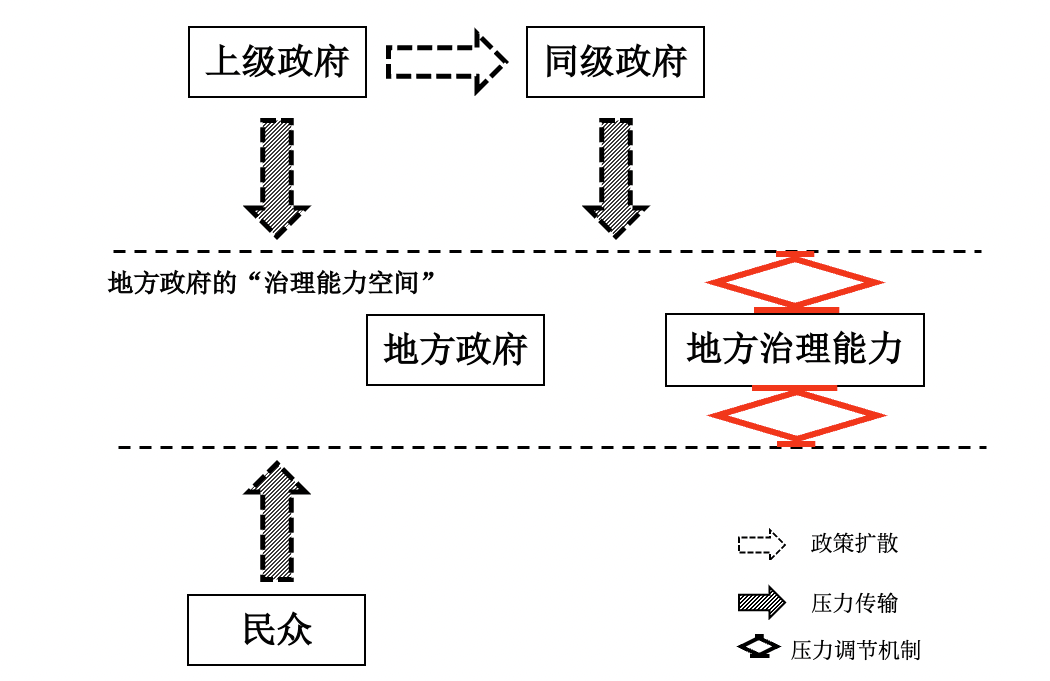
\includegraphics[width=1\linewidth]{../figures/figure2} \caption{“能力空间”与压力型体制}\label{fig:unnamed-chunk-1}
\end{figure}

\hypertarget{ux5b9eux8bc1ux68c0ux9a8cux4ee52021ux5e74ux6625ux8282ux671fux95f4ux5404ux5730ux7684ux75abux60c5ux9632ux63a7ux653fux7b56ux4e3aux4f8b}{%
\section{实证检验:以2021年春节期间各地的疫情防控政策为例}\label{ux5b9eux8bc1ux68c0ux9a8cux4ee52021ux5e74ux6625ux8282ux671fux95f4ux5404ux5730ux7684ux75abux60c5ux9632ux63a7ux653fux7b56ux4e3aux4f8b}}

下文中,笔者以2021年春节期间疫情防控政策在中国各地的差异化制定为案例,来剖析和验证地方政治治理能力对``压力型体制''运行的影响。疫情防控是2021年中国各地政府工作的核心任务。元旦和春节期间,由于人员流动性大,聚集性活动活动多,进口冷链食品和货物物流增大,做好``两节''期间新型冠状病毒的疫情防控工作更是各地任务的重中之重。春节期间疫情防控政策是考察``压力型体制''运行的典型案例,疫情期间,各地的政策目标十分明确,整个社会经济系统围绕当地党委政府的指挥棒运行,党政部门是既是指挥员,又是组织员和作战员 (\protect\hyperlink{ref-YangXueDong2021}{杨雪冬, 2021})。它的典型性还在于从中央到省再到各个地级市直至基层村(社区)都发布了有关``春节期间新型冠状病毒的疫情防控工作''的政策文本,而且不同层级、同一层级的不同地域的地方政府的政策文本存在较大的差异。这给我们衡量``压力型体制''在不同层级和不同地域的运行机制和逻辑以及识别``压力型体制''的影响变量和压力来源提供了充分的研究数据。与此同时,各地政府治理能力是决定疫情应对效果的关键因素(\protect\hyperlink{ref-YangXueDong2021}{杨雪冬, 2021}),其中在疫情预防阶段,数字政府能力尤为关键,它决定着一个地方的政府能否通过大数据等技术对人口流动和疫情防控进行精准把握和治理。这也给笔者考察地方治理能力尤其是数字治理能力对压力型体制运行的影响提供了绝佳的机会窗口。

\hypertarget{ux7814ux7a76ux8bbeux8ba1}{%
\subsection{研究设计}\label{ux7814ux7a76ux8bbeux8ba1}}

具体来说,本文尝试回答两个研究问题:首先,中国不同层级和地域的地方政府在2021年春节期间疫情防控政策上是否受到压力型体制的影响?具体表现为是否存在``层层加码''的现象。进一步的,哪些因素影响着他们的政策加码程度?笔者尝试通过对2021年春节期间疫情防控政策在中国各地的差异化制定的分析,来考察``压力型体制''在不同层级和不同地域的运行机制和逻辑,在此基础上笔者还进一步识别了``压力型体制''的影响变量和压力来源。笔者首先使用基于自然语言处理等方法对已有政策文本进行编码,再使用描述性统计的方式考察各地各层级的``层层加码''现象;之后借助回归分析对影响变量和压力来源进行识别和检验。

\hypertarget{ux7814ux7a76ux5047ux8bbe}{%
\subsection{研究假设}\label{ux7814ux7a76ux5047ux8bbe}}

据此,笔者提出本文的研究假设:

对于第一个研究问题,笔者提出研究假设1:

\textbf{H1:中国不同层级和地域的地方政府在2021年春节期间疫情防控政策上存在``层层加码''的现象;}

对于第二个研究问题,笔者提出研究假设2:

\textbf{H2: 地方政府的治理能力影响着当地的政策加码程度;}

\textbf{H2.1: 地方政府的数字治理能力越高,当地的政策加码程度越小;}

\textbf{H2.2: 地方政府的医疗能力越高,当地的政策加码程度越小。}

\hypertarget{ux53d8ux91cfux8bbeux7f6eux548cux6570ux636eux6765ux6e90}{%
\subsection{变量设置和数据来源}\label{ux53d8ux91cfux8bbeux7f6eux548cux6570ux636eux6765ux6e90}}

本研究的因变量是2021年春节期间疫情防控政策的加码程度,笔者对于因变量的处理分为两个部分:首先,笔者借助网络爬虫从政府网站、政府公众号和政务服务平台等数据源获取了全国293个地级市2021年春节期间的疫情防控政策;在拿到数据后,笔者使用机器编码和人工查核相结合的方式对目标政策进行编码处理,将目标政策分为``有条件自由流动''(1)、``健康报备''(2)、``核酸检测''(3)、``健康监测''(4)、``居家健康监测''(5)和``居家隔离''(6)六种类型。需要强调的是,笔者关注和编码的政策是各地针对来自\textbf{低风险地区}前往\textbf{城市地区}人群的疫情管控政策。选择低风险地区是因为社会各界对来自\textbf{中高风险}人员的管制意见较为一致,均采用严格的措施围堵疫情,而在对于来自\textbf{低风险地区}的人员管制意见差异较大,因此在制定对\textbf{低风险地区}人员的疫情管制时,地方政府会面对更大更复杂的压力;选择\textbf{城市地区}是因为中央政策明确规定了返回农村地区的防控政策\footnote{请参见国家卫生健康委员会网页:\url{http://www.nhc.gov.cn/jkj/dongt/202101/4378bd2dd76b4d9a8d995660e90fb4a6.shtml}} ,地方政府的加码空间较少,而中央对城市地区的管控政策没有明确规定。

本文的核心自变量是地方的治理能力,笔者主要关注和疫情防控相关的数字政府治理能力和医疗能力。笔者使用清华大学数据治理中心2021年发布的《中国数字政府发展研究报告》中对中国主要城市政府的数字治理能力评估的指数。这一指数侧重于分析政府利用数字化平台提供公共服务、开展政民互动的能力。该测评设置平台管理、数据开放、政务服务、政民互动四项二级指标,分别衡量数字政府发展各类功能载体的健全性、便利性、安全性等特征。在地方政府的医疗能力上笔者使用的是该地级市的医院床位数,该数据和诸如该地的国民生产总值等控制变量均整理自各地的统计年鉴。

本文的还考察了上级政府、同级政府和民众等压力来源对地方政府的压力,笔者使用地级市所在省份政策颁布前一个月(2020年12月)的新型冠状病毒确诊数量作为上级政府压力的代理变量。同级政府的压力分成两种情况,如果该地级市是副省级城市或省会城市,笔者使用同等级城市2020年12月新型冠状病毒确诊数量的平均值作为同级政府压力的代理变量;如果该地级市是一般的城市,笔者使用同省的其他城市2020年12月新型冠状病毒的确诊数量作为政府压力的代理变量。各地各层级2020年12月新型冠状病毒的确诊数量的数据来源均整理自当地卫健委。笔者使用关键词``疫情''的百度搜索指数在2020年12月的环比增长数量作为民众压力的代理变量。\footnote{请参见百度指数网页:\url{https://zhishu.baidu.com/}}

\hypertarget{ux591aux5c42ux7ea7ux4e0dux540cux5730ux5730ux65b9ux57dfux653fux5e9cux95f4ux7684ux5c42ux5c42ux52a0ux7801ux73b0ux8c61ux7ecfux9a8cux8bc1ux636e}{%
\subsection{多层级、不同地地方域政府间的``层层加码''现象:经验证据}\label{ux591aux5c42ux7ea7ux4e0dux540cux5730ux5730ux65b9ux57dfux653fux5e9cux95f4ux7684ux5c42ux5c42ux52a0ux7801ux73b0ux8c61ux7ecfux9a8cux8bc1ux636e}}

从下表中我们很容易看到,省级政府提出防控政策的严格程度平均说来都超过了中央提出的防疫政策,市级政府提出防控政策的严格程度平均说来都超过了省级政府提出的防疫政策,即从中央到地级市层级,2021年春节期间的防疫政策呈现出越向基层越严格的``层层加码''态势。

具体来说,省一级加码最多的是吉林省,要求所有``非中高风险地区返(来)吉人员须持3日内新冠病毒核酸检测阴性证明。''\footnote{具体请参见请参见《关于加强春节期间返(来)吉人员管理与服务做好新冠肺炎疫情防控工作的通知》\url{http://www.jl.gov.cn/zw/tzgg/gsgg/gg/202102/t20210201_7932090.html}}。 市一级加码最多的是以山东德州为代表的地级市,这些地方政府要求从低风险地区返回的民众,进行14天居家健康监测。

\begin{table}[!h]

\caption{\label{tab:unnamed-chunk-2}中央、省和地级市疫情防控政策比较}
\centering
\begin{tabular}[t]{ccccccc}
\toprule
\multicolumn{1}{c}{ } & \multicolumn{3}{c}{省级防控政策} & \multicolumn{3}{c}{市级防控政策} \\
\cmidrule(l{3pt}r{3pt}){2-4} \cmidrule(l{3pt}r{3pt}){5-7}
中央防控政策 & 均值 & 最大值 & 最小值 & 均值. & 最大值. & 最小值.\\
\midrule
1 & 1.23 & 3 & 1 & 1.81 & 5 & 1\\
\bottomrule
\end{tabular}
\end{table}

为了更加形象的展示不同地区在疫情防控政策上的加码情况,笔者在东、中、西和东北部各选取了一个省,具体地说,东部选取了浙江省,中部选取了河南省,西部选取了青海省,东北部选取了吉林省来详细比较他们的加码差异。

从下表数据笔者发现,在空间分布上,压力型体制仍旧是一个全国性的体制,防疫政策加码的情况在除浙江省外的中、西和东北广泛存在。而且和现有理论的发现一致,防疫政策加码的情况在空间存在上不平衡的特点 (\protect\hyperlink{ref-YangXueDong2012}{杨雪冬, 2012})。笔者还汇报了各省的省级数字治理能力指数,对比各省数字治理能力指数与疫情防控措施的加码程度可以发现,和经典理论不同的是,这种不平衡性似乎和是否处在经济起飞阶段并没有很强的相关性,而是和地方政府的数字治理能力更加相关。

\begin{table}[!h]

\caption{\label{tab:unnamed-chunk-3}东、中、西、东北地区个别省份疫情防控政策比较}
\centering
\begin{tabular}[t]{cccccc}
\toprule
省份 & 省级防控政策 & 市均值 & 市最大值 & 市最小值 & 省级数字治理能力指数\\
\midrule
浙江 & 1 & 1.00 & 1 & 1 & 37.2\\
山西 & 1 & 2.23 & 5 & 1 & 25.3\\
青海 & 1 & 2.70 & 5 & 1 & 19.3\\
吉林 & 3 & 3.20 & 4 & 3 & 28.2\\
\bottomrule
\end{tabular}
\end{table}

\textbf{由此笔者验证了本文的第一个研究假设:中国不同层级和地域的地方政府在2021年春节期间疫情防控政策上存在``层层加码''的现象,在层级上,地级市政府加码最多,在空间上,数字治理能力弱的地区加码最多。}

\hypertarget{ux80fdux529bux7a7aux95f4ux653fux5e9cux80fdux529bux4e0eux52a0ux7801ux7a0bux5ea6ux7684ux7ecfux9a8cux8bc1ux636e}{%
\subsection{``能力空间'':政府能力与加码程度的经验证据}\label{ux80fdux529bux7a7aux95f4ux653fux5e9cux80fdux529bux4e0eux52a0ux7801ux7a0bux5ea6ux7684ux7ecfux9a8cux8bc1ux636e}}

笔者继续检验本文的第二个研究假设,即检验影响地方政府政策加码程度的原因,在检验经典理论的基础上,笔者着重识别和检验了地方政府的治理能力尤其是数字治理能力的影响。

\begin{figure}[h]
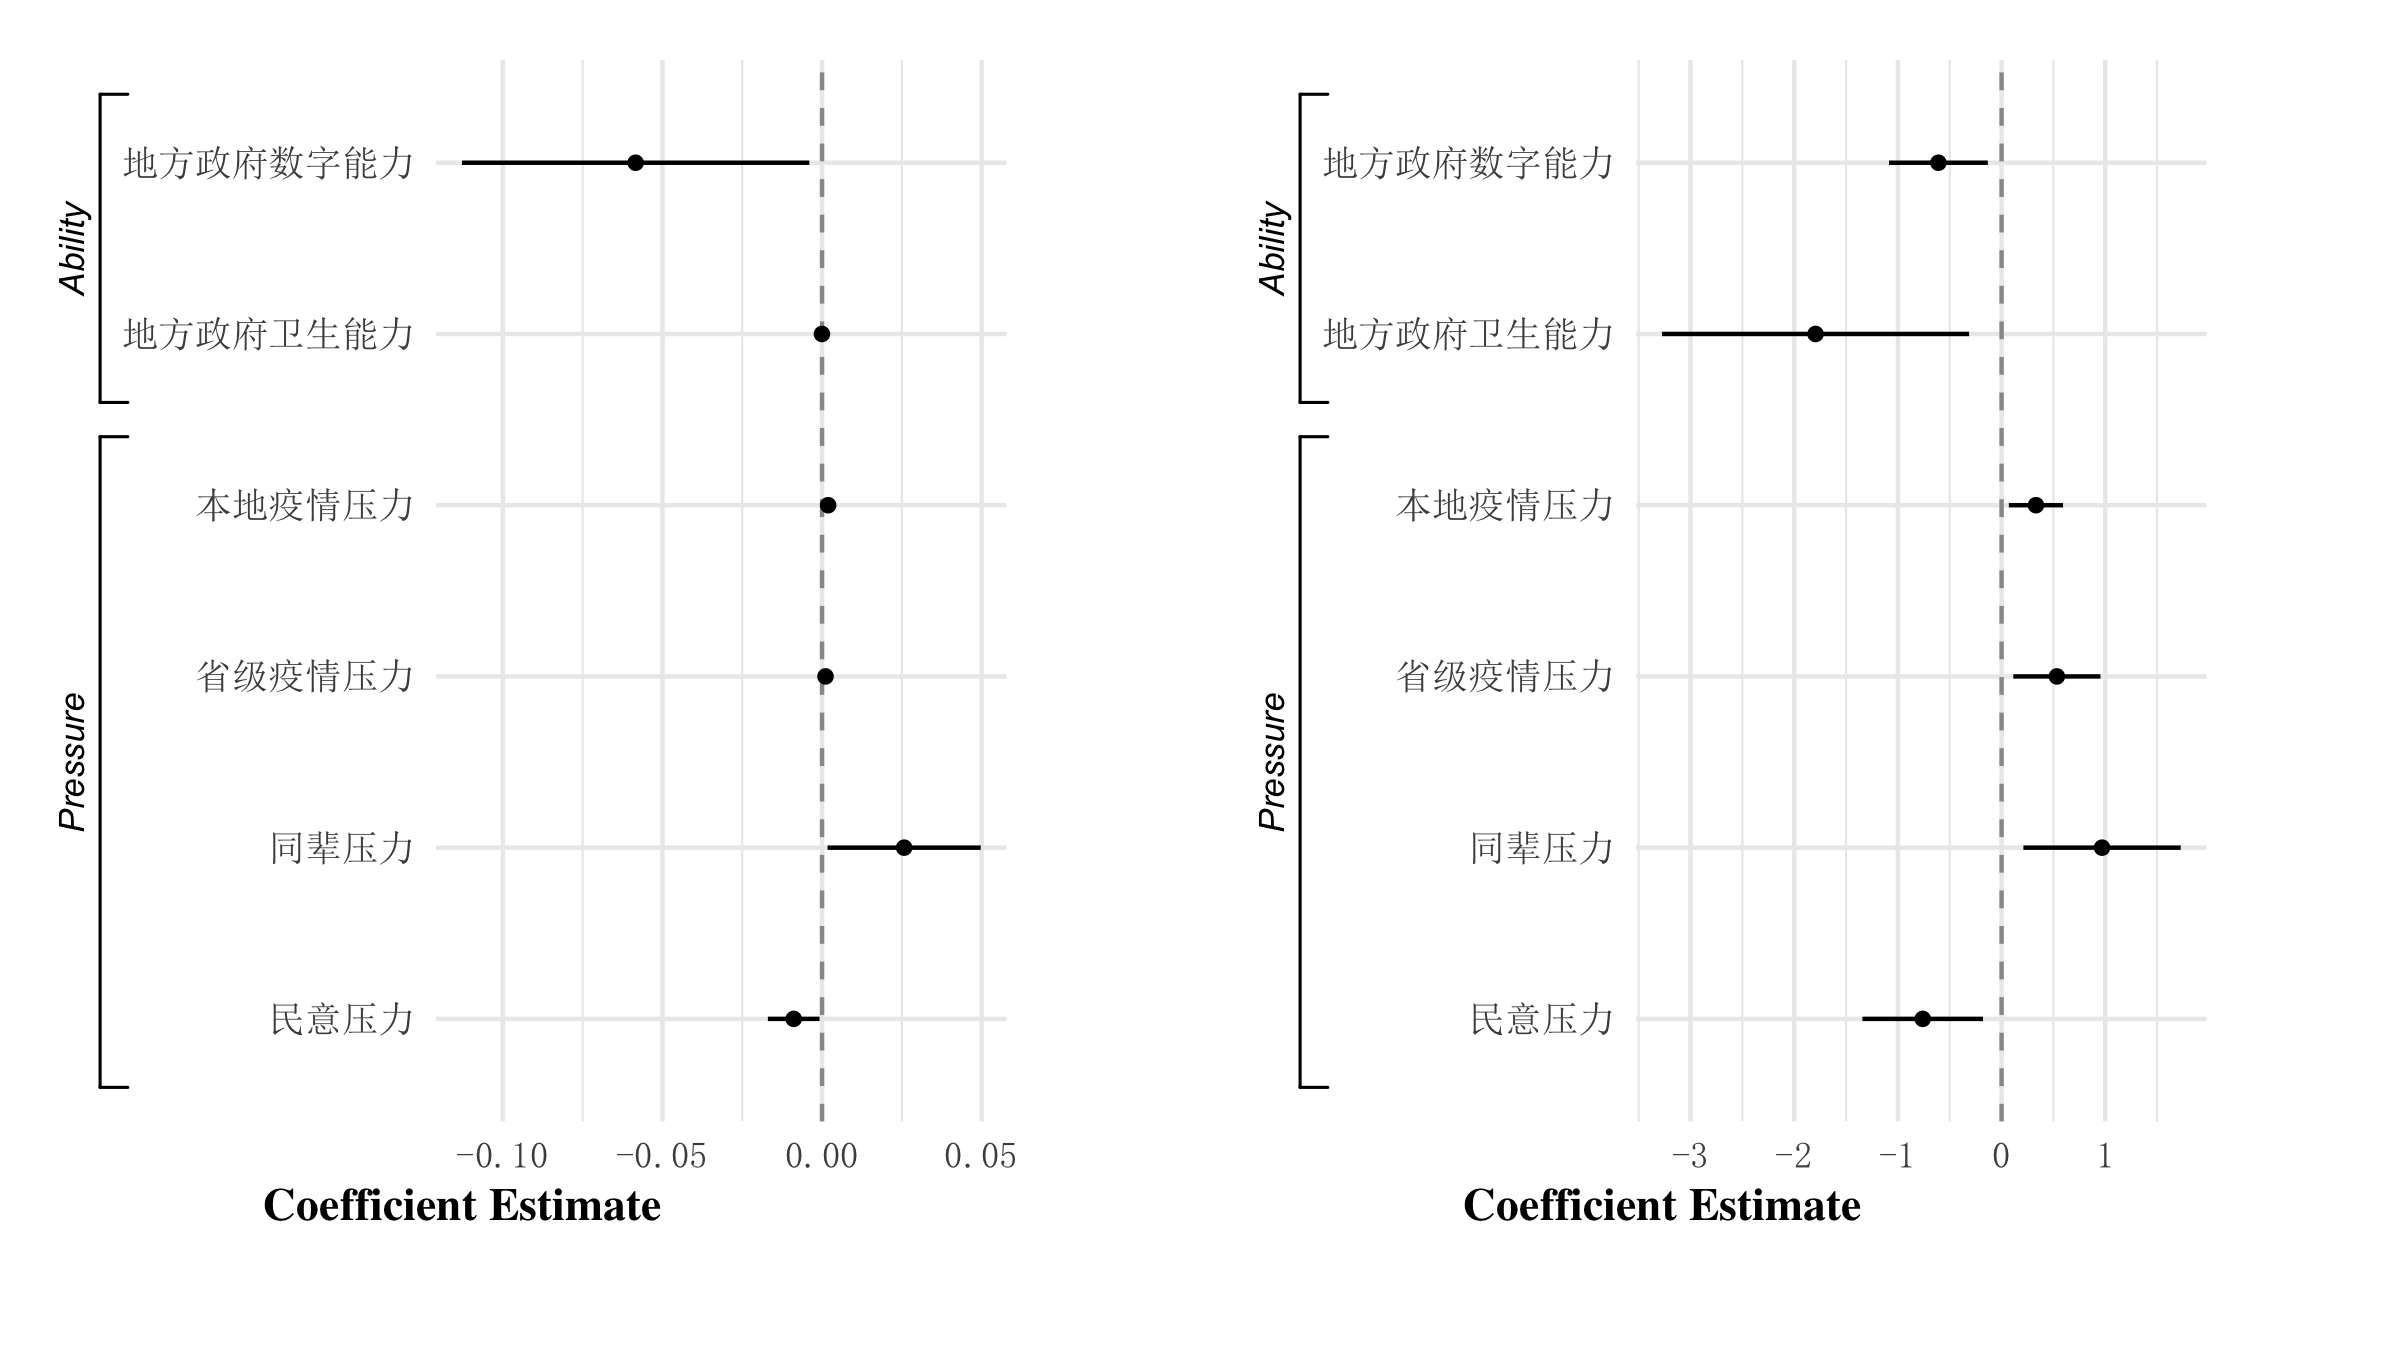
\includegraphics[width=1\linewidth]{../figures/figure1} \caption{回归结果}\label{fig:unnamed-chunk-5}
\end{figure}

根据上图回归分析的结果,笔者发现,经典理论中的四个压力来源对地方政府疫情防控政策的加码程度仍有较强的解释力,本地疫情压力、同级政府压力、上级政府压力和民众压力对地方政府疫情防控政策的加码程度仍有显著影响:在控制其他变量的前提下,本地疫情越严重,地方政府疫情防控政策加码越多;和本地同级城市疫情越严重,地方政府疫情防控政策加码越多;本地所在省份疫情越严重,地方政府疫情防控政策加码越多;民众压力越大,地方政府疫情防控政策加码越少。

在此基础上,笔者识别和检验了地方政府的治理能力尤其是数字治理能力的影响,回归分析发现,地方政府的数字治理能力和卫生能力对地方政府疫情防控政策加码程度仍有显著影响:在控制其他变量的前提下,地方政府的数字治理能力越强,地方政府疫情防控政策加码越少;地方政府的卫生能力越强,地方政府疫情防控政策加码越少。即,治理能力是地方政府面对各方压力的减压阀,治理能力越强的地方政府的行政自主性即``能力空间''就越大,从而能够较为灵活的处理多方压力和政策加码。

在对变量进行标准化处理后,我们可以比较不同自变量对因变量的影响程度。通过上右图的比较,笔者发现,地方的治理能力尤其是卫生能力,在所有自变量中对地方政府疫情防控政策的加码程度影响最大;地方的数字治理能力对地方政府疫情防控政策的加码程度也有较大影响。

\hypertarget{ux603bux7ed3ux4e0eux8ba8ux8bba}{%
\section{总结与讨论}\label{ux603bux7ed3ux4e0eux8ba8ux8bba}}

近年来,作为国家治理的核心环节,地方治理受到学者广泛的关注。压力型体制作为对现实的理论描绘,得到了国内外学者的较高认同 ,不仅生动的描述了中国地方治理的压力和动力,还由于其理论的整体性,能够对``目标责任制''、``项目制''和``行政发包制'' 等一些富有解释力的概念进行较好地整合。

中国共产党第十八次全国代表大会以来,党和政府推动了一系列重大的政治体制改革,``强监督、弱激励、硬指标''的地方治理氛围,深刻得改变了压力型体制的运行环境。在这一改革进程中,``压力型体制''的表现更趋明显,甚至已经被官方话语所接纳。虽然压力型体制仍然表现出生动的描述力和较强的解释力,但是面对新的制度环境和新的现象依旧存在解释力上的不足。

本研究在梳理已有理论的基础上,结合地方治理能力和数字政府建设等理论视角,提出压力型体制下``能力空间''的概念。笔者认为,地方政府的治理能力使得他们在各界压力下还能保留一定的自主性空间,而这一自主性空间的大小是由地方政府的治理能力的强弱决定的。

本研究以以2021年春节期间疫情防控政策在中国各地的差异化制定为案例,剖析和验证了地方政治治理能力对``压力型体制''运行的影响。通过实证分析,笔者发现,经典理论中的同级、上级和民众对地方政府的政策加码程度均有显著影响,其中同级和上级压力对政策加码程度有显著的正向影响,而民众压力对有显著的负向影响。在检验经典理论的基础上,笔者着重识别和检验了地方政府的治理能力尤其是数字治理能力的影响,笔者发现,地方政府的数字治理能力和卫生能力对地方政府疫情防控政策加码程度有明显的``减压阀''作用,治理能力越强的地方政府的行政自主性即``能力空间''就越大,从而能够较为灵活的处理多方压力和政策加码。

本文不仅利用实证数据和方法对``压力型体制''这一经典理论进行实证检验,发现在十八大之后的政治体制变革中,``压力型体制''对中国地方治理的实践仍然有较强的解释力;还发现地方政府治理能力对``压力型体制''运行的``减压阀''效应,提出了``能力空间''与``有自主性的压力型体制''的观点,对``压力型体制''在新时代进行了理论修正与检验。需要说明的是,本文也存在明显的不足:首先,由于数据的限制,笔者仅对加码行为进行了``中央-省-地级市''层面的分析,而对原有理论中``压力型体制表现得更加突出''的县级政府 (\protect\hyperlink{ref-YangXueDong2012}{杨雪冬, 2012}) 本文并没有足够的数据来进行实证检验;其次,通过大样本的数据分析虽然能够在总体上发现相关性,但是在影响机制上的探索有限。地方政府治理能力对压力型体制下地方自主性的具体影响机制还有待后续研究进一步完善。

\newpage

\hypertarget{ux53c2ux8003ux6587ux732e}{%
\section*{参考文献}\label{ux53c2ux8003ux6587ux732e}}
\addcontentsline{toc}{section}{参考文献}

\hypertarget{refs}{}
\begin{CSLReferences}{1}{0}
\leavevmode\hypertarget{ref-Ahlers2019}{}%
AHLERS A L, 2019. Political Inclusion in Contemporary {China}{[}M{]}. {Taylor \& Francis}.

\leavevmode\hypertarget{ref-Edin2003}{}%
EDIN M, 2003. State Capacity and Local Agent Control in {China}: {CCP} Cadre Management from a Township Perspective{[}J{]}. China Q., : 35.

\leavevmode\hypertarget{ref-Guo2020}{}%
GUO B, 2020. A {Partocracy} with {Chinese Characteristics}: {Governance System Reform} under {Xi Jinping}{[}J{]}. Journal of Contemporary China, 29(126): 809--823.

\leavevmode\hypertarget{ref-MontinolaEtAl1995}{}%
MONTINOLA G, QIAN Y, WEINGAST B R, 1995. Federalism, {Chinese} Style: The Political Basis for Economic Success in {China}{[}J{]}. World politics, : 50--81.

\leavevmode\hypertarget{ref-QianXu1993}{}%
QIAN Y, XU C, 1993. The {M}-Form Hierarchy and {China}'s Economic Reform{[}J{]}. European Economic Review, 37(2-3): 541--548.

\leavevmode\hypertarget{ref-Schubert2020}{}%
SCHUBERT A, 2020. Local {Governance} in {China} {} {A Critical State}-of-the {Art Review}{[}Z{]}(2020--12).

\leavevmode\hypertarget{ref-Shue1990}{}%
SHUE V, 1990. The Reach of the State: Sketches of the {Chinese} Body Politic{[}M{]}. {Stanford University Press}.

\leavevmode\hypertarget{ref-TsuiWang2004}{}%
TSUI K, WANG Y, 2004. Between Separate Stoves and a Single Menu: Fiscal Decentralization in {China}{[}J{]}. The China Quarterly, : 71--90.

\leavevmode\hypertarget{ref-YangYan2018}{}%
YANG X, YAN J, 2018. Top-Level Design, Reform Pressures, and Local Adaptations: An Interpretation of the Trajectory of Reform since the 18th {CPC Party Congress}{[}J{]}. Journal of Chinese Governance, 3(1): 25--48. DOI:\href{https://doi.org/10.1080/23812346.2018.1428075}{10.1080/23812346.2018.1428075}.

\leavevmode\hypertarget{ref-FengShiZheng2014}{}%
冯仕政, 2014. 政治市场想象与中国国家治理分析{}{}兼评周黎安的行政发包制理论{[}J{]}. 社会, 34(6): 70--84.

\leavevmode\hypertarget{ref-ZhouXueGuang2009}{}%
周雪光, 2009. 基层政府间的 {《共谋现象》}{}{}一个政府行为的制度逻辑{[}J{]}. 开放时代, 12: 40--55.

\leavevmode\hypertarget{ref-ZhouXueGuangLianHong2012}{}%
周雪光, 练宏, 2012. 中国政府的治理模式: 一个 {《控制权》} 理论{[}J{]}. 社会学研究, 5(69): r93.

\leavevmode\hypertarget{ref-ZhouFeiZhou2009}{}%
周飞舟, 2009. 锦标赛体制{[}J{]}. 社会学研究, 3(5): 4--77.

\leavevmode\hypertarget{ref-ZhouLiAn2014}{}%
周黎安, 2014a. 行政发包制{[}J{]}. 社会, 34(6): 1--38.

\leavevmode\hypertarget{ref-ZhouLiAn2014a}{}%
周黎安, 2014b. 再论行政发包制: 对评论人的回应{[}J{]}. 社会, 34(6): 98--113.

\leavevmode\hypertarget{ref-ZhouLiAnEtAl2015}{}%
周黎安, 刘冲, 厉行, 等, 2015. {《层层加码》} 与官员激励{[}J{]}. 世界经济文汇, 1(01): 1--15.

\leavevmode\hypertarget{ref-MengTianGuangLiFeng2015}{}%
孟天广, 李锋, 2015. 网络空间的政治互动: 公民诉求与政府回应性{}{}基于全国性网络问政平台的大数据分析{[}J{]}. 清华大学学报 (哲学社会科学版), 30(3): 17--29.

\leavevmode\hypertarget{ref-ZhangWenCui2021}{}%
张文翠, 2021. 基层政府政绩目标设置博弈与压力型体制异化{}{}基于北方七个地市的实地调研{[}J{]}. 公共管理学报, : 1--12.

\leavevmode\hypertarget{ref-PengBoZhaoJi2019}{}%
彭勃, 赵吉, 2019. 从增长锦标赛到治理竞赛: 我国城市治理方式的转换及其问题{[}J{]}. 内蒙古社会科学 (汉文版), 1: 63--67.

\leavevmode\hypertarget{ref-JingYueJin2018}{}%
景跃进, 2018. 中国农村基层治理的逻辑转换{}{}国家与乡村社会关系的再思考{[}J{]}. 中共浙江省委党校学报, 1.

\leavevmode\hypertarget{ref-ZhuGuangNanEtAl2012}{}%
朱光楠, 李敏, 严敏, 2012. 公务员公共服务动机对工作投入的影响研究{[}J{]}. 公共行政评论.

\leavevmode\hypertarget{ref-LiZhen2014}{}%
李振, 2014. 推动政策的执行: 中国政治运作中的工作组模式研究{[}J{]}. 政治学研究, 2.

\leavevmode\hypertarget{ref-LiZhenEtAl2020c}{}%
李振, 王浩瑜, 孙宇飞, 等, 2020. {《条块并举》}发包制下的基层治理{}{{以T区乡镇政府的精准扶贫工作为例}}{[}J{]}. 公共行政评论, 13(03): 102-117+196-197.

\leavevmode\hypertarget{ref-YangXueDong2012}{}%
杨雪冬, 2012. 压力型体制: 一个概念的简明史{[}J{]}. 社会科学, 11(4): 12.

\leavevmode\hypertarget{ref-YangXueDong2018}{}%
杨雪冬, 2018. {地方治理的逻辑}{[}M{]}. {北京}: {社会科学文献出版社}.

\leavevmode\hypertarget{ref-YangXueDong2021}{}%
杨雪冬, 2021. 疫情防控检验着共同体的韧性{[}J{]}. 环球时报, : 015.

\leavevmode\hypertarget{ref-WangYuLei2016}{}%
王雨磊, 2016. 数字下乡:农村精准扶贫中的技术治理{[}J{]}. 社会学研究, 31(06): 119--142+244.

\leavevmode\hypertarget{ref-RongJingBen1998a}{}%
荣敬本, 1998. 从压力型体制向民主合作体制的转变: 县乡两级政治体制改革{[}M{]}. {中央编译出版社}.

\leavevmode\hypertarget{ref-ChenJiaJian2013}{}%
陈家建, 2013. 项目制与基层政府动员{}{}对社会管理项目化运作的社会学考察{[}J{]}. 中国社会科学, 2: 64--79.

\leavevmode\hypertarget{ref-ChenJiaJian2015}{}%
陈家建, 2015. 督查机制: 科层运动化的实践渠道{[}J{]}. 公共行政评论, 2(5): 21.

\leavevmode\hypertarget{ref-HuangXiaoChun2017}{}%
黄晓春, 2017. 当前城市基层政府改革的深层挑战{}{}基于机制分析的视角{[}J{]}. 江苏行政学院学报, 3.

\end{CSLReferences}

\end{document}
